To demonstrate when in the developing process we will try to apply PRT, we will make a timeline. The timeline contains all the phases of a software development process. The software development processes are different for each kind of approach. For this research we will make a timeline using the SCRUM development process.
\section{Scrum} 
\subsection{Definition of Scrum}
SCRUM is a development process named to the rugby method of play. In rugby it means that a formation will group together to gain the ball as fast as possible. For the developing this means that a group of people work in short sprints to realize the desired software product as soon as safe as posible. The scrum development team consists of the following members: product-owner, developers and scrum masters. The product owner makes sure the organising part of the developing will get enough attention. The scrum master makes sure that the developers make the right decisions and to make sure the overall process will go in the right way. The other members will make the actual product. 
\subsection{Phases of Scrum}
SCRUM contains 3 kind of phases. The planning and closure phases consist of knowing the input and output of the project. These phases are just organising phases, so not much developing will be made. The development will take place during the sprints which can be divided in developing, wrapping, reviewing and adjusting. This is a continuous process which will finish once the project is in the closure phase. Developing is where the programming will be done, then wrapping is done to combine all the elements of the development process, reviewing is done to make sure if the process is working well and adjusting is the phase to improve the implemented functions. Sprints are in cycles, so after the adjusting phase, the developing phase will be the next phase, so that the cycle is complete.

\begin{figure}[h]
\begin{center}
	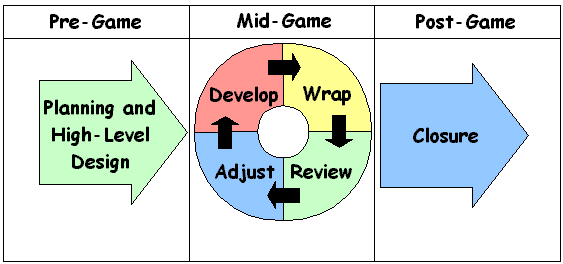
\includegraphics[width=0.5\textwidth]{Figures/diagram01.png}
\end{center}
	\caption{phases of scrum}

\end{figure}

\section{When to Perfrom Regress Test using Scrum} Now we can choose where in the development process PRT will take place. The planning and closure phases are no good for PRT, because these phases are just organising phases. So PRT will be done during the sprints. Research has been done to show that automated regression tests during the daily builds will greatly improve the quality of the product \cite{Future_of_Scrum}. Regression testing was done during the merging phase of the scrum. In the end they made sure that everything was tested for regressions yet again, to make sure the product was ready to ship.

\section{Other possibility}Another research appointed one person of the developing group to continuously watch over the quality of the software product \cite{Fully_Distributed_Scrum}. This person is an active member of the team and watches all the members of the developing team. This method provides a way to deal with any issues that could come up during the process. The appointed person will directly try to deal with issues coming up by the members of the developing team. By appointing this person, the quality of the producht is watched the whole time during the project. Instead of comparison to the other research where PRT is done during the merge phase. This research proved that the quality of the development got a much higher average score compared to other similar development products. So appointing one tester who only has the task to watch over the quality by testing and for our sake performing regression tests, has an improved effect on the overall process.

